% ---
% titre: Les messageries utilisées par les jeunes en Suisse (lecture d'un diagramme en barres)
% theme: FA
% chapitre: Diagrammes
% sous_chapitre: Lire, interpréter et réaliser	
% niveau: [10e]
% type: EVAL
% tags: [c-diagramme-colonnes,c-lecture-diagramme,c-addition,p-question-TS]
% difficulte: 1
% corrige: true
% source: ZHAW Psychologie des Médias, étude JAMES 2024
% ---

\question
L'étude suisse JAMES (2024) a demandé à 1\,137 jeunes de 12 à 19 ans à quelle fréquence ils utilisent différentes messageries. Le diagramme ci-dessous indique, pour chaque messagerie, la part des jeunes (en \%) pour chaque fréquence d'utilisation.
 
\vspace{30pt}
\begin{center}
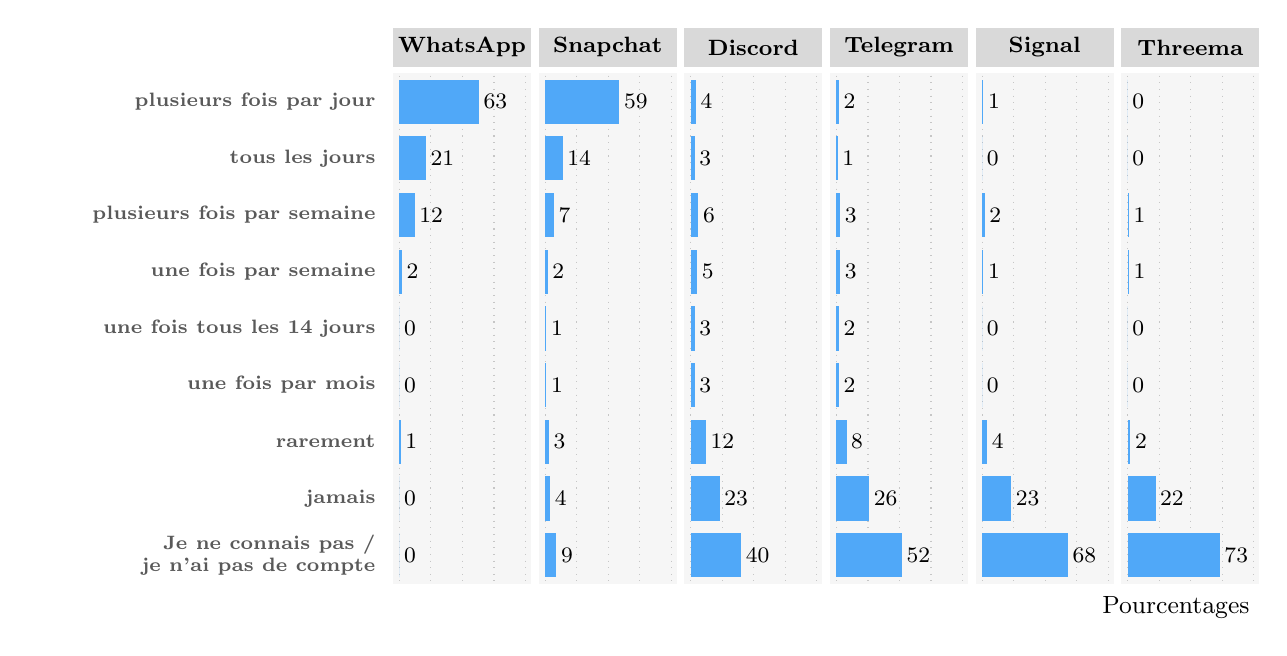
\begin{tikzpicture}
  \def\lw{4.6}    % largeur de la zone des étiquettes (cm)
  \def\pw{1.75}   % largeur d'un panneau
  \def\pp{1.85}   % pas entre deux panneaux
  \def\rh{0.72}   % hauteur d'une ligne
  \def\sc{0.016}  % 1 % = 0,016 cm
  \definecolor{barre}{RGB}{80,168,248}
  % en-têtes, fonds et lignes pointillées (0, 25, 50, 75, 100 %)
  \foreach \nom [count=\k from 0] in {WhatsApp,Snapchat,Discord,Telegram,Signal,Threema}{
    \pgfmathsetmacro{\xo}{\lw+\pp*\k}
    \fill[gray!30] (\xo,0.08) rectangle (\xo+\pw,0.58);
    \node[font=\footnotesize\bfseries] at (\xo+0.5*\pw,0.33) {\nom};
    \fill[gray!7] (\xo,0) rectangle (\xo+\pw,-9*\rh);
    \foreach \g in {0,25,50,75,100}{
      \draw[gray!45, dotted] (\xo+0.08+\g*\sc,-0.03) -- (\xo+0.08+\g*\sc,-9*\rh+0.03);
    }
  }
  % légende de l'axe horizontal
  \node[anchor=east, font=\small] at (\lw+6*\pp-0.1,-9*\rh-0.3) {Pourcentages};
  % étiquettes des lignes
  \foreach \lab [count=\r] in {plusieurs fois par jour, tous les jours, plusieurs fois par semaine, une fois par semaine, une fois tous les 14 jours, une fois par mois, rarement, jamais, Je ne connais pas / je n'ai pas de compte}{
    \node[anchor=east, text width=4.3cm, align=right, font=\scriptsize\bfseries, text=black!65] at (\lw-0.1,-\r*\rh+0.5*\rh) {\lab};
  }
  % barres et valeurs
  \foreach \wa/\sn/\di/\te/\si/\th [count=\r] in {63/59/4/2/1/0, 21/14/3/1/0/0, 12/7/6/3/2/1, 2/2/5/3/1/1, 0/1/3/2/0/0, 0/1/3/2/0/0, 1/3/12/8/4/2, 0/4/23/26/23/22, 0/9/40/52/68/73}{
    \foreach \v [count=\k from 0] in {\wa,\sn,\di,\te,\si,\th}{
      \pgfmathsetmacro{\xo}{\lw+\pp*\k+0.08}
      \fill[barre] (\xo,-\r*\rh+0.08) rectangle (\xo+\v*\sc,-\r*\rh+\rh-0.08);
      \node[anchor=west, font=\footnotesize, inner sep=1.5pt] at (\xo+\v*\sc,-\r*\rh+0.5*\rh) {\v};
    }
  }
\end{tikzpicture}
\end{center}
{\footnotesize\raggedleft Source : \textcopyright\ 2024 ZHAW Psychologie des Médias (étude JAMES 2024).\par}
 
 \begin{parts}
\vspace{40pt}\part[1] Quelle messagerie est utilisée plusieurs fois par jour par le plus grand nombre de jeunes ? Quel pourcentage de jeunes l'utilise ainsi ?
 
\vspace{5pt}
\begin{tcolorbox}[enhanced jigsaw, interior hidden, colframe=box, parbox=false]%
Réponse : 
\sol{\vspace{20pt}}{C'est WhatsApp, utilisée plusieurs fois par jour par 63\,\% des jeunes. \textbf{(0,5\,pt)} pour la messagerie, \textbf{(0,5\,pt)} pour le pourcentage}
\end{tcolorbox}
 
\vspace{20pt}\part[1\half] Quelle part des jeunes utilise Snapchat tous les jours ou plus souvent ?
 
\vspace{5pt}{\footnotesize\raggedleft Espace pour ta démarche et tes calculs\par}
\begin{solutionorgrid}[80pt]
\vspace{5pt}
\og Plusieurs fois par jour \fg : 59\,\% et \og tous les jours \fg : 14\,\% \hfill\textbf{(0,5\,pt)}
 
\vspace{10pt}$59 + 14 = 73$ \hfill\textbf{(0,5\,pt)}
\end{solutionorgrid}
 
\begin{tcolorbox}[enhanced jigsaw, interior hidden, colframe=box, parbox=false]%
Réponse : 
\sol{\vspace{20pt}}{73\,\% des jeunes utilisent Snapchat tous les jours ou plus souvent. \textbf{(0.5pt)}}
\end{tcolorbox}
 
\vspace{20pt}\part[1\half] Sam affirme : \og Plus de la moitié des jeunes ne connaissent pas Signal ou n'ont pas de compte. \fg{} A-t-il raison ? Justifie ta réponse à l'aide d'une donnée du diagramme.
 
\vspace{5pt}{\footnotesize\raggedleft Espace pour ta démarche\par}
\begin{solutionorgrid}[80pt]
\vspace{5pt}
Lecture dans la colonne \og Signal \fg de la ligne \og Je ne connais pas / je n'ai pas de compte \fg : 68\,\% \hfill\textbf{(0.5pt)}
 
\vspace{10pt}La moitié correspond à 50\,\% et $68 > 50$. \hfill\textbf{(0.5pt)}
\end{solutionorgrid}
 
\begin{tcolorbox}[enhanced jigsaw, interior hidden, colframe=box, parbox=false]%
Réponse : 
\sol{\vspace{20pt}}{Oui, Sam a raison : 68\,\% des jeunes ne connaissent pas Signal ou n'ont pas de compte, ce qui est plus que la moitié. \textbf{(0.5pt)}}
\end{tcolorbox}

\vspace{20pt}\part[1\half] Sur 100 jeunes, combien utilisent WhatsApp au moins une fois par semaine ?

\vspace{5pt}{\footnotesize\raggedleft Espace pour ta démarche et tes calculs\par}
\begin{solutionorgrid}[100pt]
\vspace{5pt}
Lignes à prendre en compte : \og plusieurs fois par jour \fg{} (63\,\%), \og tous les jours \fg{} (21\,\%), \og plusieurs fois par semaine \fg{} (12\,\%) et \og une fois par semaine \fg{} (2\,\%). \hfill\textbf{(0,5\,pt)}

\vspace{10pt}$63 + 21 + 12 + 2 = 98$ \hfill\textbf{(0,5\,pt)}
\end{solutionorgrid}

\begin{tcolorbox}[enhanced jigsaw, interior hidden, colframe=box, parbox=false]%
Réponse : 
\sol{\vspace{20pt}}{98 jeunes sur 100 utilisent WhatsApp au moins une fois par semaine. \textbf{(0,5\,pt)}}
\end{tcolorbox}
\end{parts}